\documentclass[a4paper]{article}

\usepackage[utf8]{inputenc}
\usepackage[portuguese]{babel}
\usepackage{a4wide}
\usepackage[pdftex]{hyperref}
\usepackage{graphicx}
\usepackage{wrapfig}
\usepackage{amsmath}
\usepackage{verbatim}
\usepackage{caption}
\usepackage{subcaption}
\usepackage{float}
\usepackage{blochsphere}



\begin{document}

\begin{titlepage}
\begin{center}



\includegraphics[width=0.4\textwidth]{logo.jpg}\\[0.5cm]

\vspace{10mm}

{\huge Universidade do Minho - Escola de Engenharia}\\[0.5cm]

{\large Relatório do trabalho prático de Computação Gráfica}\\[0.5cm]

\vspace{10mm}

% Title
\rule{\linewidth}{0.5mm} \\[0.4cm]
{ \huge \bfseries Fase 1 – Primitivas Gráficas \\[0.4cm] }
\rule{\linewidth}{0.5mm} \\[1.5cm]

% Author and supervisor
\noindent
\begin{minipage}{0.4\textwidth}
  \begin{flushleft} \large
    \emph{Autores :}\\
    Daniel Maia \textsc{(A77531)}\\
    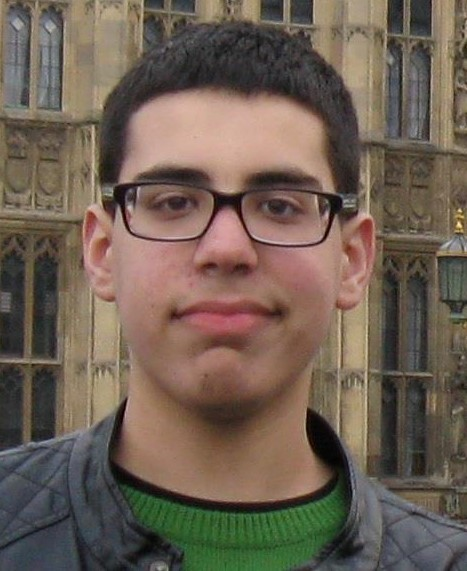
\includegraphics[width=1.5cm]{daniel.jpg}\break
    Diogo Silva\textsc{(A78034)}\\
    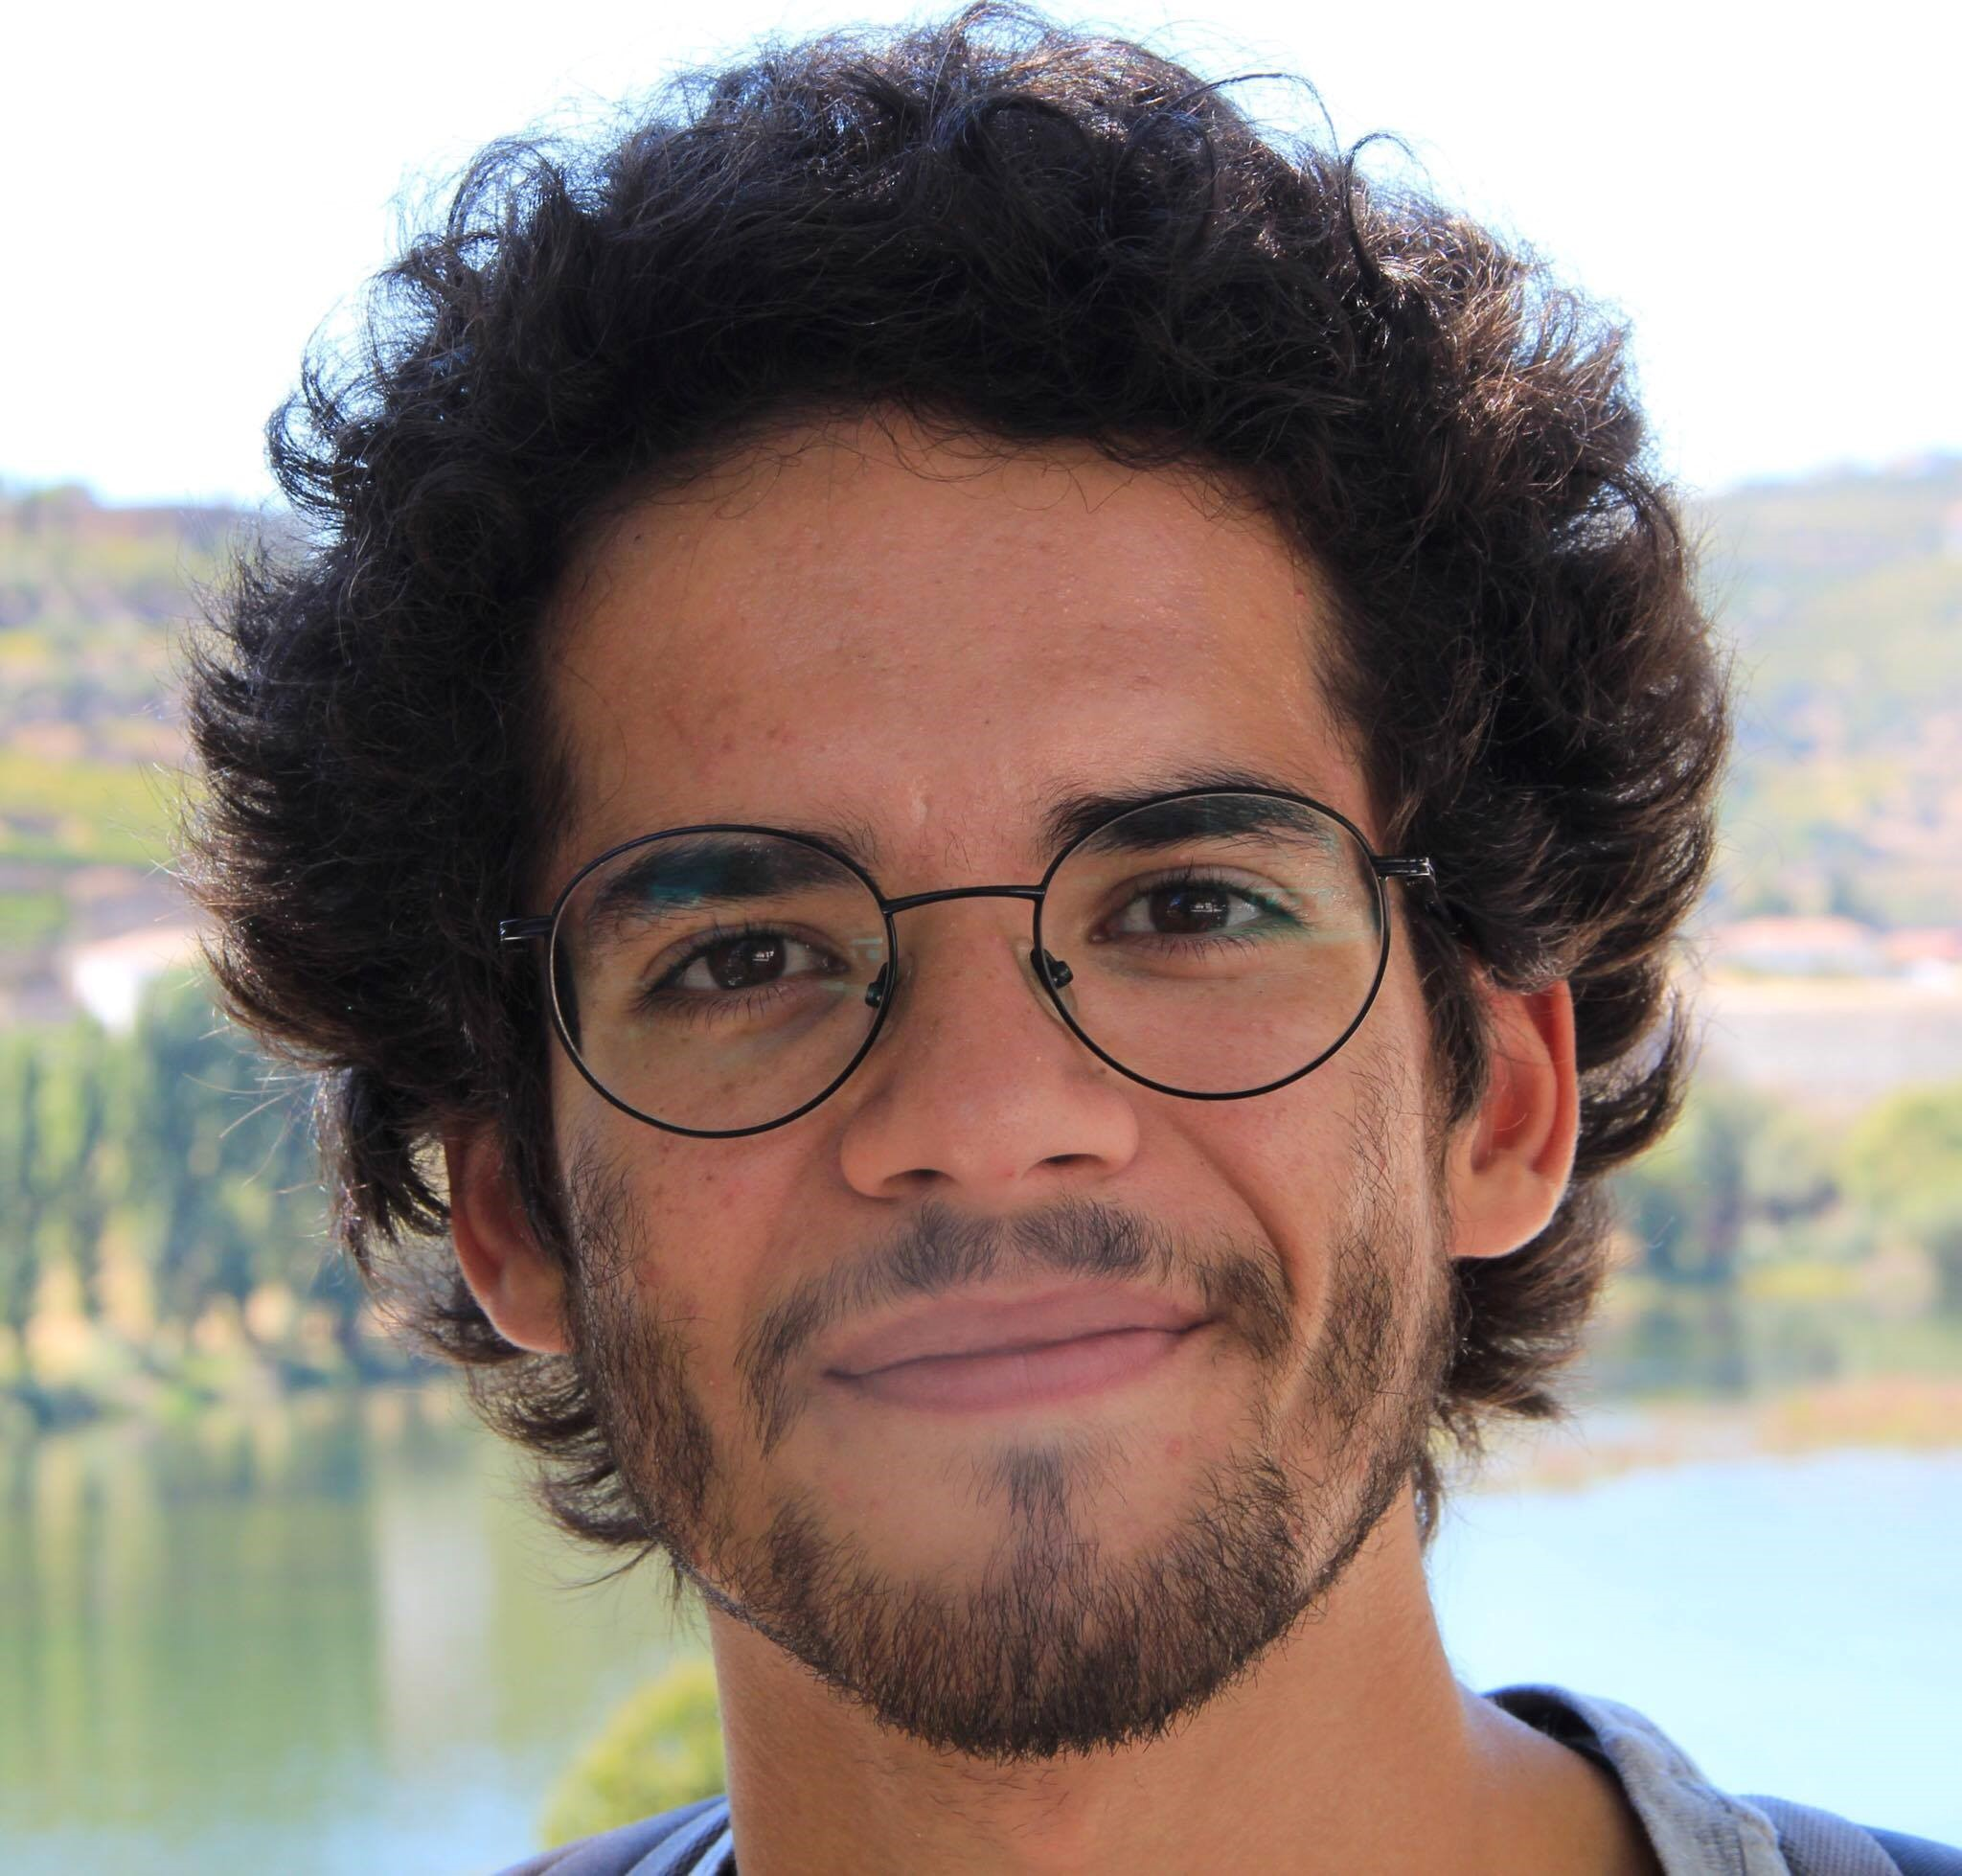
\includegraphics[width=1.5cm]{afonso.jpg}\break
    Marco Silva\textsc{(A79607)}\\
    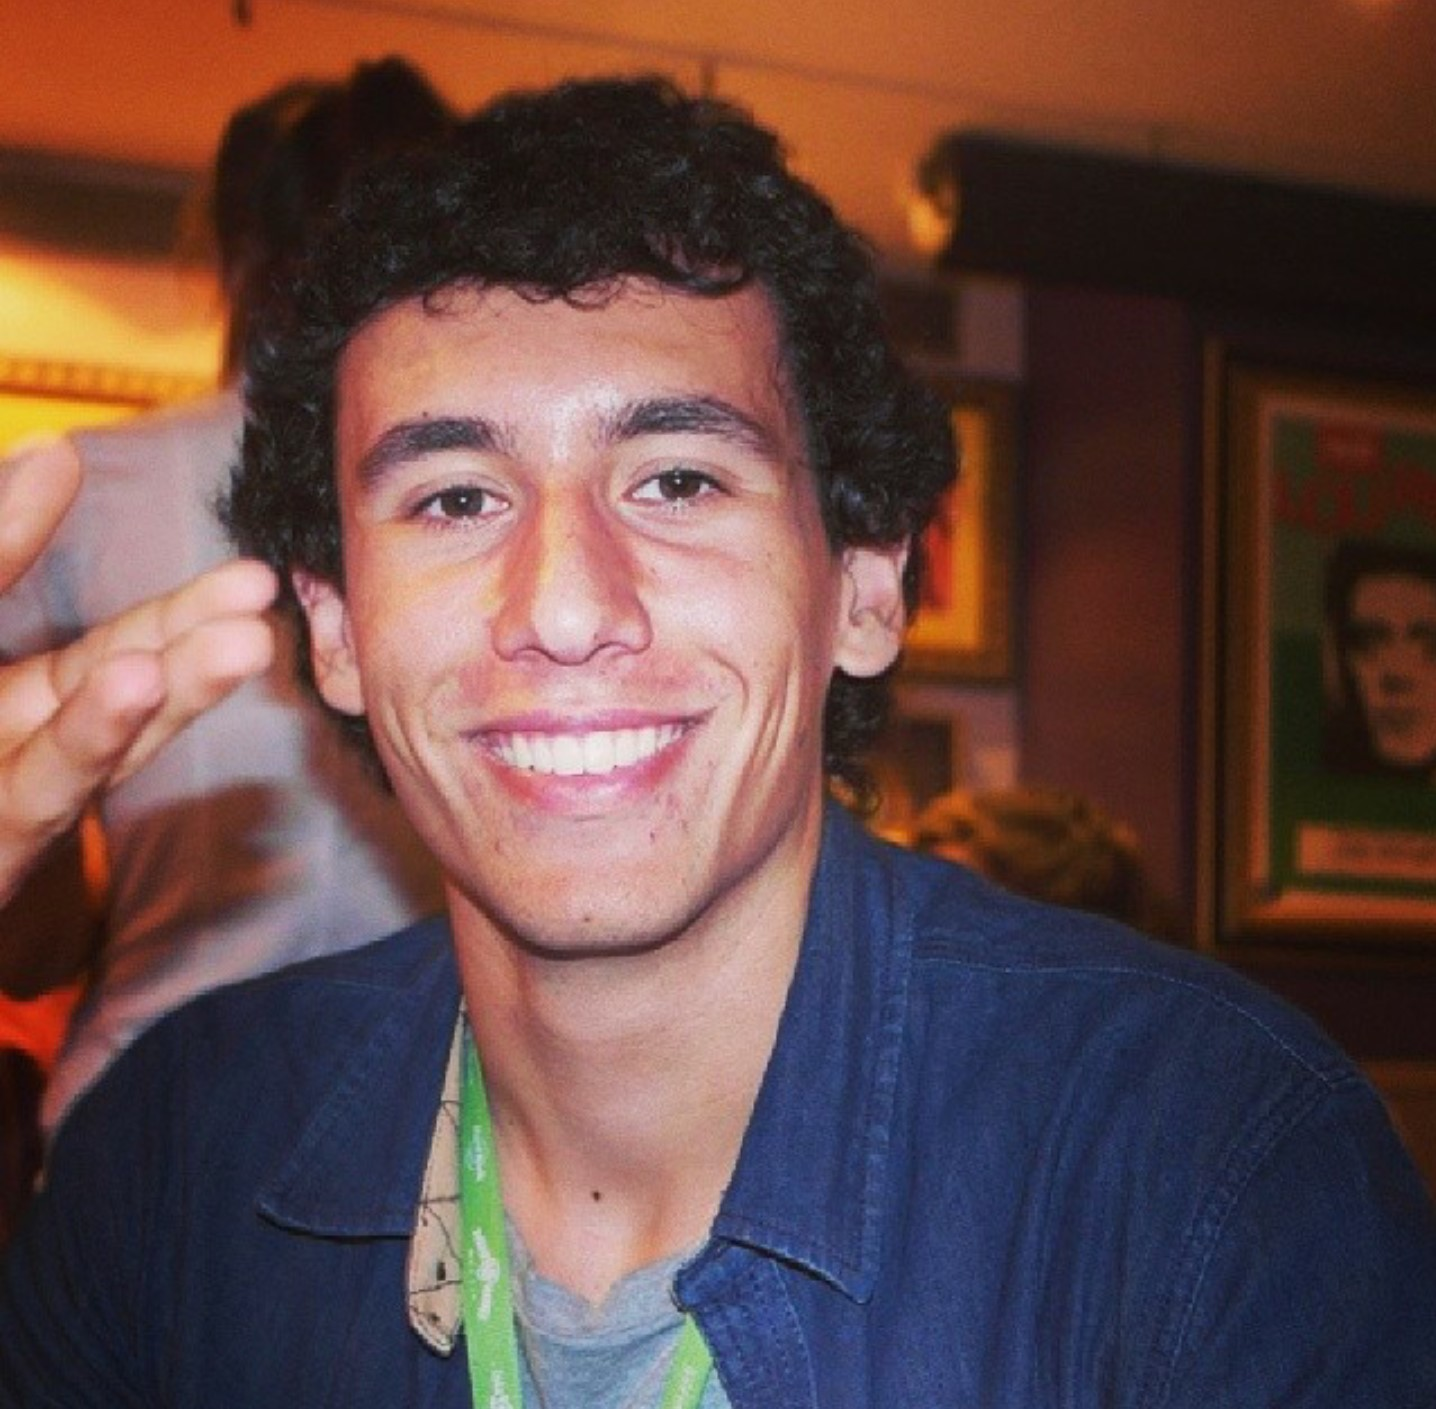
\includegraphics[width=1.5cm]{marco.jpg}\break
  \end{flushleft}
\end{minipage}%
\vfill

% Bottom of the page
{\large Versão 1.0 \\ \today}

\end{center}
\end{titlepage}


\begin{abstract}

\hspace{3mm}

\end{abstract}

\pagebreak
\tableofcontents

\pagebreak

% ===================================================
\section{Introdução}


% ===================================================
\section{Preliminares}


% ===================================================
\section{Descrição do Trabalho e Análise de Resultados}

\subsection{Introdução}



\subsection{Generator}

\hspace{3mm} Antes de abordar qualquer pormenor mais técnico relacionado com a geração dos pontos para as diversas figuras a desenhar, é importante explicitar que foi definida uma norma para a escrita nos ficheiros que irão representar as figuras abaixo descritas. Foi então estabelecido que em cada uma das linhas teremos as 3 coordenadas em formato cartesiano com a ordem x, y e z, separadas por espaços ficando assim em cada linha toda a informação necessária para a representação de um ponto.

\subsubsection{Plano} % nº de triângulos = 2

\hspace{3mm} Trata-se de um quadrado com um comprimento N passado por argumento na linha de comandos. Como tal, é necessário apenas determinar quatro pontos com os quais se poderá definir dois triângulos. O plano está centrado em XZ, logo, os pontos seguem o formato (x, 0, z), x e z sendo \pm \[\frac{N}{2}\]. Para manter a semântica do OpenGL, dois destes pontos terão um duplicado no ficheiro plano.3d. %atenção que aqui não podemos dizer diretamente o nome do ficheiro uma vez que este pode ser especificado pelo utilizador

\begin{figure}[h!]
\centering
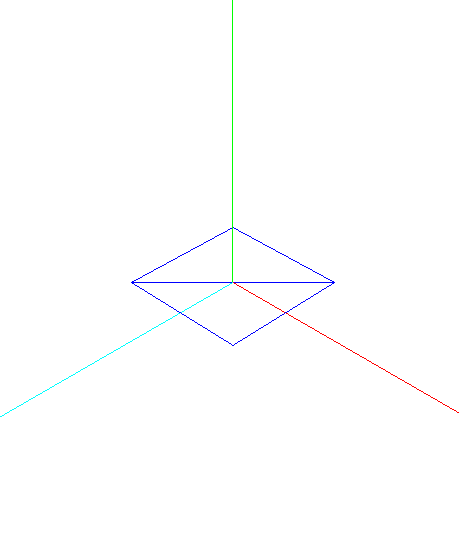
\includegraphics[width=7cm]{plane.png}
\caption{Exemplo de um plano.}
\label{fig:plane}
\end{figure}

\subsubsection{Box} % nº de triângulos = 6 * (2^divisions)

\subsubsection{Cone} % nº de triângulos = ( 2 * (stacks * slices) ) + slices

\subsubsection{Esfera} % nº de triângulos = 2 * stack * slices

\hspace{3mm} Para a construção da esfera, inicialmente foram estudadas as várias possibilidades para a representação das coordenadas. O mais comum seria a utilização de coordenadas cartesianas mas uma vez que para o desenho da esfera pretendemos representar superfícies planas foram utilizadas coordenadas polares.

\begin{figure}[h!]
\centering
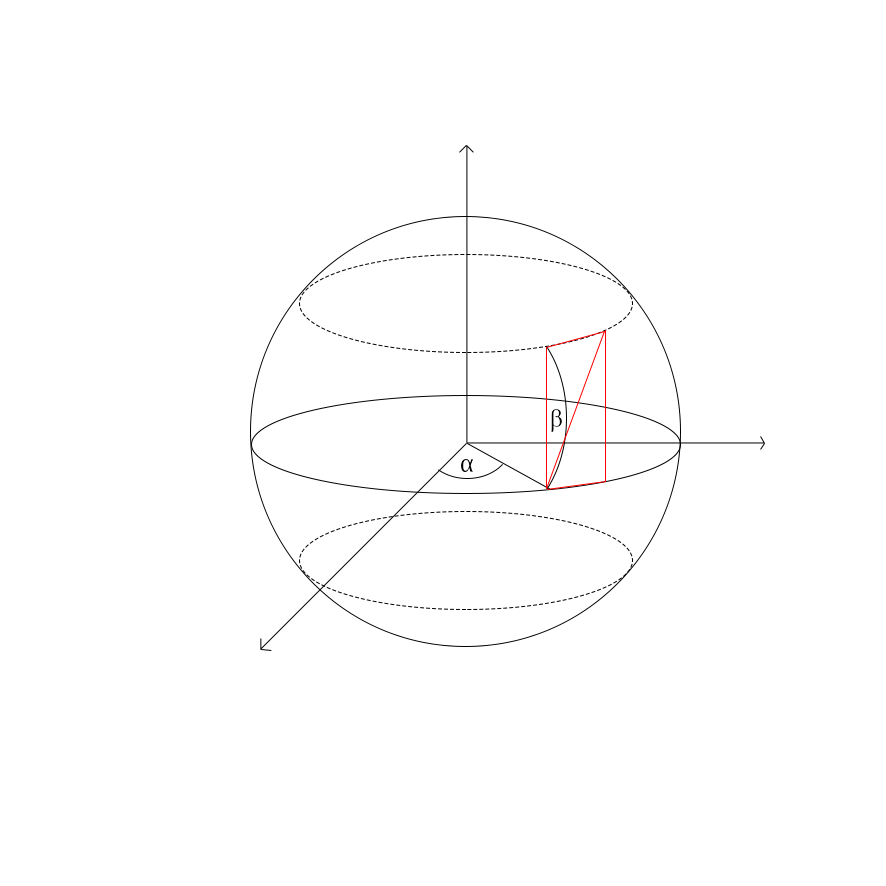
\includegraphics[width=7cm]{sphere.png}
\caption{Representação da esfera utilizando coordenadas polares e demonstração do passo iterativo de desenho de triângulos.}
\label{fig:sphere}
\end{figure}

\par Uma vez que para o desenho de qualquer figura utilizando o OpenGL, foi necessário encontrar uma estratégia que fosse eficiente para o desenho desta figura. Uma vez que, juntamente com a especificação do raio da esfera a desenhar é também fornecido o número de \emph{slices} (divisões verticais) e \emph{stacks} (divisões horizontais), conclui-se que as variações dos ângulos $\alpha$ e $\beta$ que se podem ver representados na figura acima, irão estar diretamente relacionadas com o número de \emph{slices} e \emph{stacks} respetivamente.
\par Primeiramente, são calculados os incrementos quer em $\alpha$ quer em $\beta$ com base no valor de \emph{slices} e \emph{stacks} que são necessários. No caso das \emph{slices} (correspondente ao $\alpha$ na figura), $increment1 = (2\Pi) / \emph{slices}$ uma vez que terão de ser desenhadas \emph{slices} em redor de toda a esfera enquanto que para as \emph{stacks}, $increment2 = \Pi / \emph{stacks}$. Para as \emph{stacks}, apenas é necessário percorrer $\Pi$ radianos visto que o desenho das \emph{slices} já percorrem $2\Pi$ radianos cobrindo assim por completo a superfície da esfera.
\par Tendo este raciocínio consolidado, apenas é necessário explicitar os passos a tomar em cada uma das iterações. Tendo em atenção a imagem acima apresentada, podemos ver o desenho a vermelho de dois triângulos que juntos representam um retângulo. As coordenadas destes pontos são determinadas com base nos ângulos atuais quer de $\alpha$ e $\beta$ adicionando os incrementos respetivos calculados anteriormente.
\par Este raciocínio encontra-se dentro de dois ciclos, cada um com o número de \emph{stacks} e \emph{slices} indicados.


\subsection{Engine}

\subsubsection{Formato XML}

\hspace{3mm} O formato XML surge neste projeto como "guião" da cena a ser desenhada uma vez que tem nele descrito os ficheiros de pontos que devem ser desenhados e numa fase mais avançada, instruções como \emph{translate} ou \emph{rotate}.
\par Nesta primeira fase, o ficheiro XML é bastante simples, sendo apenas constituído por uma \emph{tag} scene que por sua vez alberga a \emph{tag} model com o atributo \emph{file} que representa o nome do ficheiro de pontos a desenhar.
\par Tendo assim bem definida a estruturação do ficheiro, apenas é necessário aceder aos conteúdos deste ficheiro e extrair a informação necessária, neste caso são apenas necessários os nomes dos ficheiros de pontos.

\subsubsection{Leitura e Desenho}

\hspace{3mm} Uma vez extraída a informação necessária do ficheiro XML, pode-se proceder então ao tratamento dos ficheiros em causa. Primeiramente, estes são abertos apenas com permissões de escrita e é feita a leitura linha a linha dos mesmos.
\par Tendo em atenção à estrutura definida anteriormente destes ficheiros, para o tratamento do ficheiro foi utilizada uma função \emph{split} que dando um string, um delimitador e um vetor, procede à divisão da mesma colocando o resultado no vetor indicado.
Tendo a informação já devidamente tratada, basta apenas proceder à conversão do formato \emph{string} para \emph{float} recorrendo à função \emph{atof}. Assim, percorrendo todas as linhas do ficheiro e fornecendo os dados extraidos ao OpenGL, as figuras são construidas na sua totalidade.

% ===================================================
\section{Conclusões e Sugestões}


% ===================================================
\section{Referências}

% será que deveriamos colocar a referencia onde fui buscar a função split??

% ===================================================
\section{Anexos}

\end{document}
